\chapter{User Interface}\label{cha:interface}
This chapter describes the fundamental user interface concepts used by
XCSoar, and is intended as an overview.  More detailed descriptions
are given in following chapters.

\todonum[inline]{explain the principal display modes}

\begin{center}
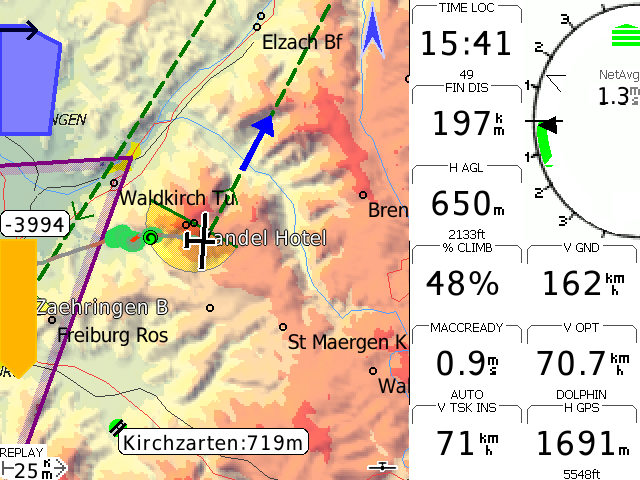
\includegraphics[angle=0,width=\linewidth,keepaspectratio='true']{figures/plain.png}
\end{center}

The XCSoar display is composed of several parts:
\begin{description}
\item[Map area] The bulk of the screen is dedicated to the GPS moving map
display. Various symbols relating to glide computer information are overlaid 
on the map area. Icons and text may appear along the lower edge of the screen
to indicate status of connected devices, operating modes etc.
\item[{\InfoBox}es] A grid of data values is displayed usually either along
the top and bottom of the screen (portrait display) or to the right of the
screen (landscape display).  These so-called {\InfoBox}es display data from the
GPS and other input devices as well as data calculated by XCSoar.
\item[Gauges]  Gauges provide instrumentation displays. All gauges are optional
and some may only have meaningful information displayed when XCSoar is
connected to a supported instrument.
\item[Button labels and menus] Hardware buttons on the device running XCSoar
can be used to bring up and navigate smaller on-screen menus that are
typically laid out such that menu items can be selected by pressing the
button adjacent to the item.  If the device has a touch screen, the menu
items can be selected by touching them.  These buttons are drawn in black
text on a green background.
\item[Status messages] Text is displayed over the map area in status message
boxes.  This text is used to present detailed information to the pilot when
certain events occur.
\item[Dialog windows] Larger dialog windows, usually containing graphics and
buttons, are used to present detailed data to the pilot regarding waypoint
details, statistics and analysis etc.
\item[Main menu] The main menu is accessible by double tapping the map area or
infoboxes as well as through gesture\gesture{Down - Up}. If the menu buttons are
not pressed after a specified time, they disappear again so as to not obscure the map area.
\end{description}

There are several ways to interact with XCSoar:
\begin{itemize}
\item Touching certain map elements
\item Touching InfoBoxes and onscreen menu buttons
\item `Gesturing', by e.g. drawing a dash from the left to the right
  on the screen (see Section \ref{sec:gestures} below).
\item `Dragging' the screen (touching the screen and moving before releasing).
\item Pressing application buttons on the device.
\item Pressing the cursor keys on the device.
\item Pressing keys or switches on an instrument connected to XCSoar.
\end{itemize}
Depending on the particular hardware used with XCSoar, not all of these methods
of interaction are possible and there may be different numbers or assignments
of buttons.

For the PC version of XCSoar, clicking the mouse over an item is equivalent to
touching it.

Since the Altair does not have a touch screen, all user interaction is performed
via physical buttons, switches or other external interface devices if connected.

\section{Button labels and menus}
The button menu is a set of buttons drawn on the screen and activated by touch
or hardware button presses.  Using buttons and the button menu is the primary
way the user interacts with XCSoar.

\begin{center}
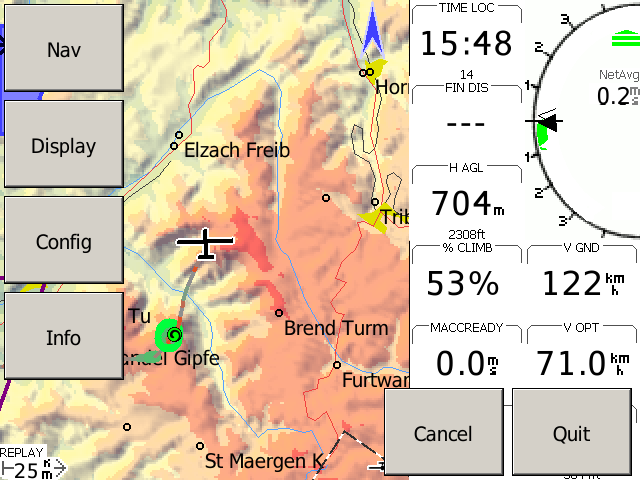
\includegraphics[angle=0,width=\linewidth,keepaspectratio='true']{figures/buttonmenu.png}
\end{center}

\subsection*{Interface basics}
The menu is organised into four different groups of functions, usually in
the form of a hierarchy.  The specific menu layout depends on the
hardware button configurations and platform, and may also be customised by the
user.

XCSoar can also accept input from external keyboards, game-pads, joysticks,
stick grip switches etc. A wide variety of functions can be assigned to these
inputs.

For Altair, there are four major menus, activated by pressing one of
the vertical strip of hardware buttons on the left of the display.
When a menu is activated, a strip of onscreen buttons appear along the 
bottom of the display.  Pressing the particular menu button again will
cycle through several pages of items.  Pressing the corresponding
horizontal button will activate that item.  At the last page, pressing
the menu button again will turn that menu off and the horizontal strip
of onscreen buttons disappear.  

On the PC version, these mode buttons are activated by the
1, 2, 3 and 4 keys.  The 6, 7, 8, 9 and 0 keys correspond to the horizontal
strip of buttons.

On the PDA version, the mode buttons are activated by the keys to the
side of the joystick/rocker button.

If the user doesn't interact with the computer for some time, the
menu will close automatically.  This menu timeout is configurable.
The escape key on PC, or the PWR/ESC button on Altair, can
also be used to close the current menu.

Menu buttons appear greyed out if the corresponding function is not available. 
For example, the ``Waypoint list'' function will appear grey if there are no waypoints loaded.

Several menu button labels have dynamic text based on context, in
order to make it clearer as to what happens when the button is
pressed.  The convention is used that a button's label describes what
will happen when the button is pressed.  For example, if the button
says \bmenu{MC Auto}, then pressing the button will turn on auto
MacCready, and the button label will then change to \bmenu{MC Manual}. 
In the menu list described below, generic labels are used.

\subsection*{Menu overview}
This section describes the default layout of the menu system on all
platforms.  The functions performed by each button are explained more
fully in following chapters.

The primary menu buttons are activated by each of the vertical strip of buttons
on Altair, from top to bottom:
\begin{jspecs}
\item[\bmenu{Nav}] Actions for navigation control, primarily cross-country
gliding tasks.
\item[\bmenu{Display}] Actions to control the display.
\item[\bmenu{Config}] Configuration of XCSoar, connected devices, and in-flight
settings.
\item[\bmenu{Info}] Activates various informational dialog windows.
\end{jspecs}

For the PC version, the keys 1, 2, 3 and 4 activate the 
corresponding menu.

\subsection*{Navigation menu (Nav)}
\jindent{\bmenut{Task}{Calc}}{ Displays the task calculator dialog. }
\jindent{\bmenut{Arm}{Start}}{ Arms the automatic task 
waypoint trigger. }
\jindent{\bmenut{Previous}{turnpoint}}{ Selects the previous/start waypoint in
the task. }
\jindent{\bmenut{Next}{turnpoint}}{ Selects the next/finish waypoint in the
task. }
\jindent{\bmenut{Waypoint}{List}}{ Displays the waypoint selector dialog. }
\jindent{\bmenut{Task}{Edit}}{ Displays the task editor. }
\jindent{\bmenus{GoTo}}{ Displays the waypoint selector dialog and activates
the GoTo mode for the selected waypoint. }
\jindent{\bmenut{Task}{Abort}}{ Aborts/resumes the current task. }
\jindent{\bmenus{Alternates}}{ Shows a list to landable alternates in the near, sorted by
by the configured aspect and distance.} 
\jindent{\bmenus{Target}}{ Displays the target dialog, which is
important for modifying AAT tasks. }

\subsection*{Display menu}
\jindent{\bmenut{Zoom}{In}}{ Zooms in the map display. }
\jindent{\bmenut{Zoom}{Out}}{ Zooms out the map display. }
\jindent{\bmenut{Zoom}{Auto}}{ Toggles automatic/manual zooming. }
\jindent{\bmenut{Mark}{Drop}}{ Drops a marker at the current glider location. }
\jindent{\bmenut{Pan}{On}}{ Activates pan map mode. }
\jindent{\bmenut{Labels}{On}}{ Displays map labels, MID labels, or none. }
\jindent{\bmenut{Trail}{Full}}{ Selects a display option out of Full,
Long, Short, Off. }
\jindent{\bmenut{Terrain}{On}}{ Toggles display of terrain. }
\jindent{\bmenut{Topography}{On}}{ Toggles display of topography. }
\jindent{\bmenut{Info}{Auto}}{  Steps through InfoBox grids.  }


\subsection*{Configuration menu (Config)}
\jindent{\bmenut{MC}{$+$}}{ Increases MacCready value. }
\jindent{\bmenut{MC}{$-$}}{ Decreases MacCready value. }
\jindent{\bmenut{MC}{Auto}}{ Toggles automatic/manual MacCready. }
\jindent{\bmenut{Flight}{Setup}}{ Displays the flight settings
(bugs/ballast/QNH) dialog. }
\jindent{\bmenut{Setup}{Wind}}{ Displays the wind settings dialog. }
\jindent{\bmenus{Vario}}{ Control of Vega intelligent variometer, this 
comprises a sub-menu. }
\jindent{\bmenut{Setup}{System}}{ Displays the XCSoar configuration dialog. }
\jindent{\bmenut{Settings}{Airspace}}{  Displays the airspace filter dialog. }
\jindent{\bmenut{Logger}{Start}}{ Turns on/off XCSoar's software IGC flight
recorder. } 
\jindent{\bmenus{Replay}}{ Displays the IGC/NMEA logger replay dialog. }
\jindent{\bmenut{Raw}{Logger}}{ Activates the raw NMEA logger (usually only used
for debugging). }
\jindent{\bmenus{Devices}}{  Displays the Device connection dialog.  }
\jindent{\bmenus{Setup Plane}}{  Displays the selection dialog for plane profiles.  }

\subsection*{Information menu (Info)}
\jindent{\bmenut{FLARM}{Radar}}{ Opens the full screen FLARM radar dialog. }
\jindent{\bmenut{METAR}{TAF}}{  Displays the METAR/TAF dialog.  }
\jindent{\bmenut{Nearest}{Airspace}}{ Displays details of the airspace nearest
to the aircraft. }
\jindent{\bmenut{Waypoint}{Details}}{ Displays the waypoint details dialog of
the active task waypoint. }
\jindent{\bmenut{Check}{List}}{ Displays the check list dialog. }
\jindent{\bmenus{Analysis}}{ Displays the analysis/statistics dialog. }
\jindent{\bmenus{Status}}{ Displays the status dialog. }
\jindent{\bmenus{Weather}}{ Displays the weather forecast dialog. }
\jindent{\bmenut{Team}{Code}}{ Opens the team code dialog. }
\jindent{\bmenut{FLARM}{Details}}{Opens the FLARM details dialog.  }
\jindent{\bmenut{Thermal}{Assistant}}{ Opens the full screen thermal assistant
dialog. }
\jindent{\bmenus{Credits}}{  Displays version information and developer team details.  }
\jindent{\bmenut{Nearest}{Waypoint}}{ Displays details of the waypoint nearest
to the aircraft. }
\jindent{\bmenut{Message}{Repeat}}{ Repeats the last status message. }


\subsection*{Variometer sub-menu (Vario) of the Configuration menu}
 The functions in this sub-menu require the Vega intelligent
variometer. The menu can only be accessed if ``Vega'' is selected as the
connected device.

\jindent{\bmenut{Airframe}{Switches}}{ Displays airframe switch values. }
\jindent{\bmenut{Setup}{Audio}}{ Adjusts volume of sounds produced by XCSoar as
well as certain speech announcements by the Vega intelligent variometer. }
\jindent{\bmenut{Manual}{Demo}}{ Activates Vega variometer manual tone demo. }
\jindent{\bmenut{Setup}{Stall}}{ Opens Vega stall monitor setup dialog. }
\todonum{what is that for?}\jindent{\bmenus{Accel}}{  }
\jindent{\bmenut{ASI}{Zero}}{ Zeros the airspeed indicator. }
\jindent{\bmenut{Accel}{Zero}}{ Levels/zeros the accelerometers. }
\jindent{\bmenus{Store}}{ Stores Vega settings to EEPROM. }
\jindent{\bmenut{Cruise}{Demo}}{ Activates Vega variometer cruise tone demo. }
\jindent{\bmenut{Climb}{Demo}}{ Activates Vega variometer climb tone demo. }

\subsection*{Pan mode sub-menu of the Display menu}
\jindent{\bmenut{Pan}{Off}}{ Turns pan mode off. }
\jindent{\bmenut{Zoom}{in}}{ Zooms in the map display. }
\jindent{\bmenut{Zoom}{out}}{ Zooms out the map display. }
\jindent{\bmenut{Nearest}{Waypoint}}{ Displays the waypoint details dialog of 
the waypoint nearest to the aircraft, or if in pan mode, nearest to the  
cross-hairs at the center of the screen. }

\subsection*{Default buttons}

When no menu is active, (so-called default mode), the horizontal row
of buttons in Altair perform the following functions (from left to right):

\begin{center}
\begin{tabular}{c c c c c c}
 PC: & 6 & 7 & 8 & 9 & 0 \\
 Altair: & F5 & F6 & F7 & F8 & F9 \\
& \bmenut{Flight}{Setup} & \bmenut{Task}{Calc} & \bmenut{Task}{Edit} &
\bmenut{Arm}{Advance} & \bmenut{Drop}{Mark} \\
\end{tabular}
\end{center}

Pressing ESC on Altair displays labels for these default menu buttons.

For all other versions in the default mode, the cursor keys perform
the following functions:
\begin{jspecs}
\item[Up key] Zoom in
\item[Down key] Zoom out
\item[Left key] Drop marker
\item[Right key] Toggle through normal/aux. InfoBoxes and Fullscreen
\item[Enter] Clear status message or suppress FLARM gauge if open and no warning
active
\end{jspecs}

For the Altair version in the default mode, the rotary knob performs
the following functions:
\begin{jspecs}
\item[Outer knob counterclockwise] Zoom in
\item[Outer knob clockwise] Zoom out
\item[Inner knob counterclockwise] (No function assigned)
\item[Outer knob clockwise] (No function assigned)
\item[Knob button press] Clear status message or acknowledge airspace warning
\end{jspecs}

In dialog forms, the rotary knob in Altair performs the role of the cursor and
enter keys:
\begin{jspecs}
\item[Outer knob counterclockwise] Up cursor
\item[Outer knob clockwise] Down cursor
\item[Inner knob counterclockwise] Left cursor
\item[Inner knob clockwise] Right cursor
\item[Knob button press] Enter key
\end{jspecs}

For Altair, the buttons along the edge of the display can be used as
alternate ways of navigating in dialogs.  The F4 key (directly above
the rotary knob) can be used as an alternate ENTER key (instead of
pressing the rotary knob) in dialogs.  The F6 and F7 keys (directly to
the right of the rotary knob) can be used to select the next or
previous page in multipage dialogs.

\subsection*{Dynamic menu labels}
Certain menu items have dynamic labels to make it clearer what happens when the
menu item is selected.  Furthermore, items that are not available are greyed
out to indicate that selecting the menu item will not do anything.

The convention used for dynamic menu labels is for the labels to display the
action that will be performed once the menu item is selected. For example 
``Lights On'' will turn the lights on, and the menu will be updated to display
``Lights Off'', which would then if pressed turn the lights off. This
convention is used throughout XCSoar.

A selection of key dynamic menu items is presented below:
\begin{description}
\item[\bmenu{Next turnpoint}]  
  Greyed out if the task is cleared, or if the active turnpoint is the
  finish. If the currently active turnpoint is the turnpoint prior to the finish, this displays  ``Waypoint finish''.
\item[\bmenu{Previous turnpoint}]  
  Greyed out if the task is cleared, or if the active turnpoint is the
  start and there are no multiple start points.  If there are multiple
  start points and the active turnpoint is the start, then this
  displays ``Cycle start'' to allow selection between the various
  start points.  If the active turnpoint is the first turnpoint after the start, this displays ``Waypoint Start''.
\item[\bmenu{Labels}]  
  This now displays ``Labels On'', ``Labels MID'' or ``Labels Off''.
\item[\bmenu{Task calculator}]  
  Greyed out if the task is cleared or in task abort.
\item[\bmenu{Arm Advance}]  
  Greyed out if Auto or Manual advance mode is active.  Displays ``Arm
  start'' when the active turnpoint is the start and the trigger is
  not armed.  Displays ``Arm Cancel'' if the trigger is armed.
  Displays ``Arm turn'' if the active turnpoint is past the start.
\item[\bmenu{Task Edit}]
  Greyed out if there is no waypoint database.
\end{description}

\section{{\InfoBox}es}

The information displayed in the {\InfoBox} fields can be selected from a
wide variety of options (listed in Chapter~\ref{cha:infobox}). These
fields can also be used to set user configurable variables, for example
the MacCready setting.

The specific number and layout of the {\InfoBox} grid depends on the
screen orientation and the device's display size.  For a 320x240 display
Pocket PC in portrait mode, there are four {\InfoBox}es above and four
{\InfoBox}es below the map display. For landscape mode, there are 9
InfoBoxes to the right of the map display.

\begin{center}
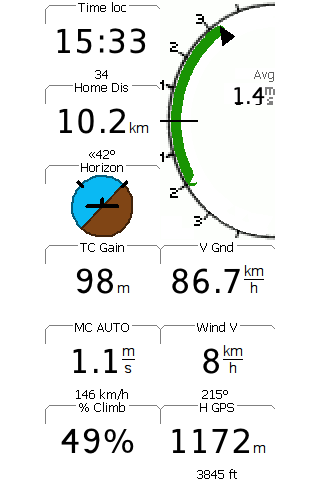
\includegraphics[angle=0,width=0.35\linewidth,keepaspectratio='true']{figures/infoboxes.png}
\end{center}

\subsection*{Screen display modes}

XC Soar allows the pilot to define various sets of InfoBoxes that are appropriate to various stages of flight (e.g. when circling in a thermal, flying between thermals, on final glide, etc.). XC Soar can be configured to automatically switch from one InfoBox display to another based on the mode of flight, or you can manually scroll through the various InfoBox displays, including a display with a full-screen map and no InfoBoxes at all.

To toggle through the various InfoBox displays, using a touchscreen:
\gesture{Right} 
or
\gesture{Left}


\subsection*{Modifying {\InfoBox} values}
(This section applies only when a touchscreen or mouse is present.)

Some {\InfoBox} values can be changed by the user by selecting (i.e. long-pressing) the
{\InfoBox} with the touchscreen or mouse.  This brings up a set of {\InfoBox}es:

\begin{description}
\item[\bmenu{Edit}]  
  Allows the pilot to adjust the {\InfoBox} setting (e.g. raise or lower the McCready setting)

\item[\bmenu{Setup}]
	Allows you to change the behavior of the setting related to the {\InfoBox} (for example, changing from Auto to Manual McCready setting mode) or choose to setup of the {\InfoBox} itself (that is, choosing \bmenu{Setup InfoBox} will display a list dialog of all available {\InfoBox}es from which to choose.

\end{description}


Examples of {\InfoBox}es that can
be adjusted include the MacCready setting, and the wind speed.

\subsection*{Changing {\InfoBox}es}
{\InfoBox}es can either be changed by calling the configuration dialog from the
menu \bmenu{Config}\blink\bmenu{Config}\blink\bmenu{Setup System} Screen 21, "InfoBox Modes" or by
performing a long press on the {\InfoBox} that should be changed. In the second case a list dialog opens,
giving you all available {\InfoBox}es to choose from.

\section{Status messages}
Status messages appear over the map area to present text for a short period of
time.  The message disappears after the time period has elapsed, and different
types of message have different periods. Additionally, status messages can be
made to disappear by acknowledging the message.  Acknowledgement is achieved by
either pressing the enter key (rotary knob on Altair), touching the status
message (on touchscreen devices) or clicking the screen (mouse enabled devices).

Additional user buttons may be assigned to a status message repeat function,
which brings up the last message again.

Typical status messages include:
\begin{itemize}
\item Airspace queries
\item Airspace warnings
\item User interface events (e.g.\ changing display modes)
\item Glide computer events (e.g.\ takeoff, turning waypoints)
\end{itemize}

Note that status messages do not appear while a dialog is on screen, the
messages are buffered and displayed as soon as the dialog is exited.

\section{Dialog windows}\label{sec:dialog-windows}

XCSoar contains several dialog windows that can be activated to bring up
additional information and are also used for more complex interactions with the
user, such as editing tasks and configuring settings.

Some dialogs simply display information, and require no user input. Other
dialogs contain data fields that can be modified or buttons that can be pressed.  

A cursor appears over the active button or data field. Pressing the up/down
arrow keys (or rotating the outer knob on Altair), the cursor will cycle
through the next or previous items. For list items and scrollable text, the
up/down arrow key moves the cursor up or down the list or text, and the
left/right arrow keys move the cursor up or down by one page in long lists.

For PDAs and PC versions, list items can be selected by touching the item (or
left-clicking with the mouse). Once a list item is selected, another touch
(left click) is equivalent to pressing the enter key.

Pressing the right/left arrow keys (or rotating the inner knob on Altair), the
data field value under the cursor can be modified. Pressing the enter key (or
pressing the rotary knob on Altair) activates the button or makes a selection
from a list.

Dialogs are typically started from the button menu.  

Many of the dialog windows have multiple pages of information and are controlled
in a consistent fashion. Press the \button{$<$} or \button{$>$} buttons to
select the next or previous page of the dialog and the \button{Close} button to
make the dialog disappear.

The escape key on a PC or the PWR/ESC button on Altair, can also be used to
close dialogs.

The user must close the dialog to return to the normal map mode. When a dialog
has been opened, the menu buttons are disabled until the dialog is closed.

In some dialogs, items that are not relevant or valid (such as AAT details when
flying a non-AAT task) are not displayed.

\todonum[inline]{This list of dialog explanations (up to 'Text entry') should
move somewhere else, because it does not explain the interface.} A summary of the
major dialogs is presented below.
\begin{description}
\item[Flight setup] Used to modify the polar of the glider both before and
during flight, as well as to set the QNH pressure
\item[Wind] Used to modify or adjust the estimated wind magnitude and direction
\item[Waypoint details] Describes a waypoint in detail and has navigation
functions such as ``GoTo'' and ``Insert in Task''
\item[Waypoint selector] Used to select a waypoint from the waypoint database
\item[Task editor] Used to edit and view cross country tasks
\item[Task calculator] Allows the pilot to see the effect of various changes to
the task on final performance
\item[Analysis] Shows several pages of analysis and statistics about the flight
\item[Status] The status dialogs give summaries of the situation of the 
aircraft, system, task, start and times
\item[Checklist] A multi-page custom checklist
\item[Configuration] Allows XCSoar and certain connected devices to be
configured
\item[Airspace colours and patterns] Configuration of colours and patterns of
airspace used on the map display
\item[Airspace filter] Controls enabling and disabling the display and warnings
of each airspace class
\item[Team code] Allows transfer of coordinates between team mates via a code
\item[Devices]  Allows setup of various external devices (e.g. glide computers, FLARM, etc.).
\item[Setup Plane]  Allows easy reconfiguration of the plane-dependant settings (e.g. polar, competition ID, etc.) by choosing from a list of previously-created plane profiles.
\end{description}

These dialogs are described in later chapters. with the exception of the
checklist, status and text entry dialogs, which are described below.

\subsection*{Checklist dialog}
The checklist dialog can display several pages of user-defined free text.
Typically this is used for checklists. It can be accessed via the menu under 
\begin{quote}
\bmenu{Info}\blink\bmenu{Check list}
\end{quote}

These checklists may include: daily inspection, preflight, outlanding,
pre-landing, radio procedures, and aircraft rigging and de-rigging
instructions.  Since the checklists may be long, the up/down keys (or rotary
knob on Altair) may be used to scroll through the text. Clicking the
\button{$<$} and \button{$>$} buttons selects the previous/next checklist.

\begin{center}
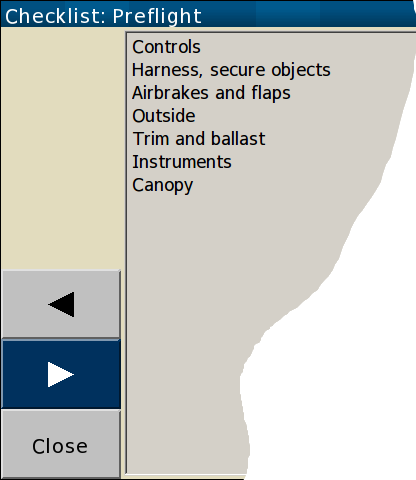
\includegraphics[angle=0,width=0.8\linewidth,keepaspectratio='true']{figures/checklist.png}
\end{center}

\subsection*{Status dialog}
The status dialog is a multi-tabular dialog giving overview information on the 
flight, system, task, rules and times. Note that the values in the Status dialog 
are static once the particular dialog page is displayed. 
That is, position, times, etc. do not update while the page is displayed. 
To see the updated values, it is necessary to select a different dialog, 
then return to the previous dialog to see the new values.

This dialog is accessed via the menu (or by gesture "S")  \gesture{Left - Down - Right - Down - Left}
\begin{quote}
\bmenu{Info}\blink\bmenu{Status}
\end{quote}

\begin{description}
\item[Flight] Shows the location of the aircraft, nearest waypoint and the
maximum height gain.
\begin{center}
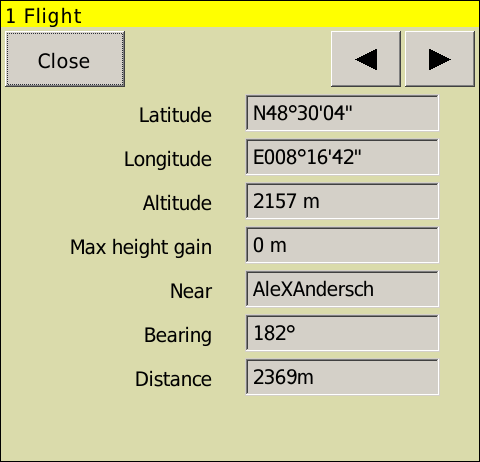
\includegraphics[angle=0,width=0.5\linewidth,keepaspectratio='true']{figures/status-aircraft.png}
\end{center}

\item[System] Shows the status of connected devices and battery levels.
\begin{center}
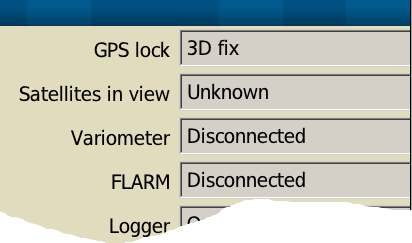
\includegraphics[angle=0,width=0.5\linewidth,keepaspectratio='true']{figures/status-system.png}
\end{center}

\item[Task] Shows the AAT times, distances achieved and remaining
and the task speeds.
\begin{center}
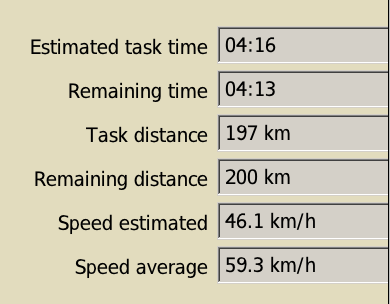
\includegraphics[angle=0,width=0.5\linewidth,keepaspectratio='true']{figures/status-task.png}
\end{center}

\item[Rules] Shows validity of start/finish according to the task rules.
\begin{center}
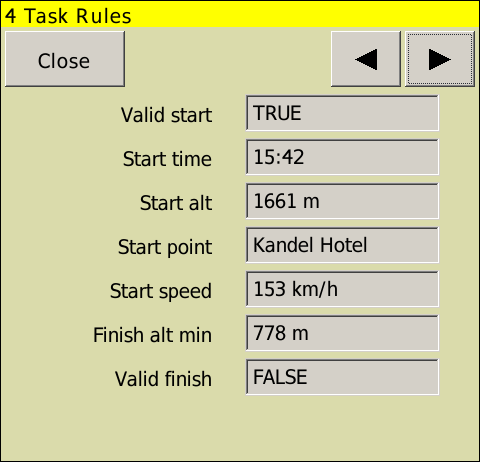
\includegraphics[angle=0,width=0.5\linewidth,keepaspectratio='true']{figures/status-rules.png}
\end{center}

\item[Times]  Shows the local time, flight time, takeoff and landing time and
the local sunset time.
\begin{center}
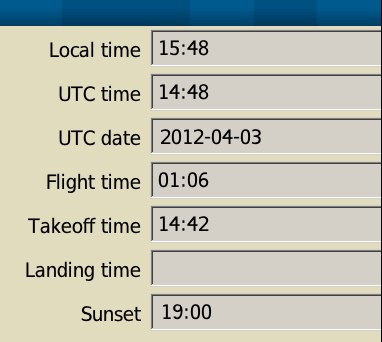
\includegraphics[angle=0,width=0.5\linewidth,keepaspectratio='true']{figures/status-times.png}
\end{center}
\end{description}

\subsection*{Text entry} \label{sec:textentry}
A text entry dialog is used for entering text.  This is used for team
code entry, setting file names, waypoint editing, as well as entering
other configuration options, such as pilot name for the logger.

Two ways of entering text are provided. See Section~\ref{sec:status} for details on customisation.

To enter text in HighScore Style, use the A+/A- buttons to adjust the character under the
cursor (underlined character). Clicking the \button{$<$} and \button{$>$} buttons move the
cursor left/right.  

\begin{center}
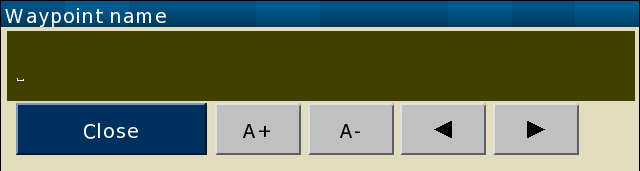
\includegraphics[angle=0,width=0.6\linewidth,keepaspectratio='true']{figures/textentry.png}
\end{center}

To enter text with the touch screen keyboard, press the letters of choice one after the other. 
In some dialogs (e.g. waypoint editing) only the next letters matching to an entry in the database 
will be shown. For deleting the last letter use the \button{$<-$} button. The
\button{Clear} button deletes all input.

\begin{center}
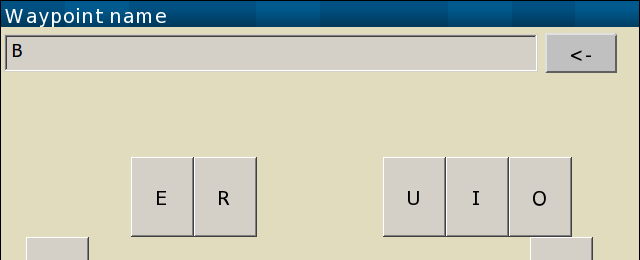
\includegraphics[angle=0,width=0.6\linewidth,keepaspectratio='true']{figures/textentry_keyboard.png}
\end{center}

Press \button{Ok} to take over, or \button{Cancel} to exit.

\section{Sounds}

XCSoar generates sounds for different events, and can be configured to
have custom sounds for any event.  See Section~\ref{sec:status} for
details on customisation.

When XCSoar is connected to the Vega intelligent variometer, it sends
commands to Vega's speech system, to give verbal cues and warnings such as:
\begin{itemize}
\item Final glide through terrain
\item Approaching/passing a task waypoint
\item Airspace warnings
\end{itemize}

\section{Screen}

Certain aspects of the look of items on the screen can be adjusted.
The most noticeable of these is whether to display {\InfoBox}es and
gauges in black on white (called inverse colours) or white on black.

For some hardware platforms, the control of the screen hardware 
brightness can be controlled from the brightness dialog
accessible from the menu:
\begin{quote}
\bmenu{Display}\blink\bmenu{Display}\blink\bmenu{Bright}
\end{quote}

Refer to the {\em Altair User's Manual} for details of the brightness
dialog.

\begin{center}
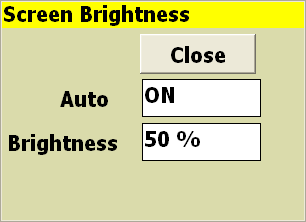
\includegraphics[angle=0,width=0.45\linewidth,keepaspectratio='true']{figures/brightness.png}
\end{center}

\section{Help system}
  A help system now provides descriptive text for properties in
  most dialogs.  When a property is selected, press and hold the
  enter button for two seconds, then release.  A window will open with
  help text describing the property.

\section{Gestures}\label{sec:gestures}
  As of version 6.0, XCSoar supports so-called mouse gestures. To activate 
  this feature go to the configuration dialog (Setup System / Interface) and
  enable it.

  To use this feature hold down the mouse button or put the finger on the 
  touchscreen, draw a certain figure and release the mouse 
  button/touchscreen. Depending on the figure that was drawn 
  a certain function is activated. A list of available gestures is 
  shown below. A figure is defined by movements of the 
  cursor in the four directions Up, Down, Left and Right. This means if 
  you hold down the mouse button, drag the mouse to the left 
  and afterwards to the top, \gesture{Left-Up} the gesture "LU" is detected,
  which stands for "Left-Up". The manual indicates an available gesture as shown
  here on the left side of the text body.


  Gestures available on the map screen:
\begin{itemize}
\item U: Zoom in
\item D: Zoom out
\item L: Toggle map mode prograde (Normal, Aux. InfoBoxes, Fullscreen)
\item R: Toggle map mode retrograde (Fullscreen, InfoBoxes, Aux., Normal)
\item DU: Show the menu
\item DR: Show the Select Waypoint dialog
\item RD: "T" opens the task dialog
\end{itemize}


  Gestures available on the FLARM radar dialog:
\begin{itemize}
\item U: Zoom in
\item D: Zoom out
\item L: Previous target
\item R: Next target
\item UD: Activate autozoom
\item DR: Open details of selected target
\item RL: Switch additional data show on the side (avg. climb/rel. altitude)
\end{itemize}

